\subsection{Corrections}

\subsubsection{Target Boiling}

Reference Sheren and Natalie paper.

Localized heating from the beam causes changes to the gas density of the target. The target does not actually boil, but the standard nomenclature for a change in target density is "boiling". By modulating the gas density, the incident beam sees a variable target thickness. This in turn affects the yield calculation.

This effect scales with the current that is on the target. We make this correction run-by-run using the average current during beam-on time during the run. This method was chosen because the average current is near constant over the coarse of a single run and the effect is approximately linear for small deviations in current. It was found that the change in density settles very quickly, so it is unnecessary to take into account beam ramp-up after beam trips.

To determine the correction, a dedicated set of runs was taken with the Left HRS spectrometer at $16.8\degree$ and $3.1GeV$. The data was taken at varying currents in order to assess the affect of the beam current on the normalized yield. By applying nominal event cuts to this data, the normalized yield was calculated. 

To determine the density correction, the normalized yields were plotted versus the beam current for that measurement. The data was then fit with a quadratic polynomial. The fit was constrained to require a correction of $1$ (no correction) at a current of $0 \mu A$.

\begin{figure}
	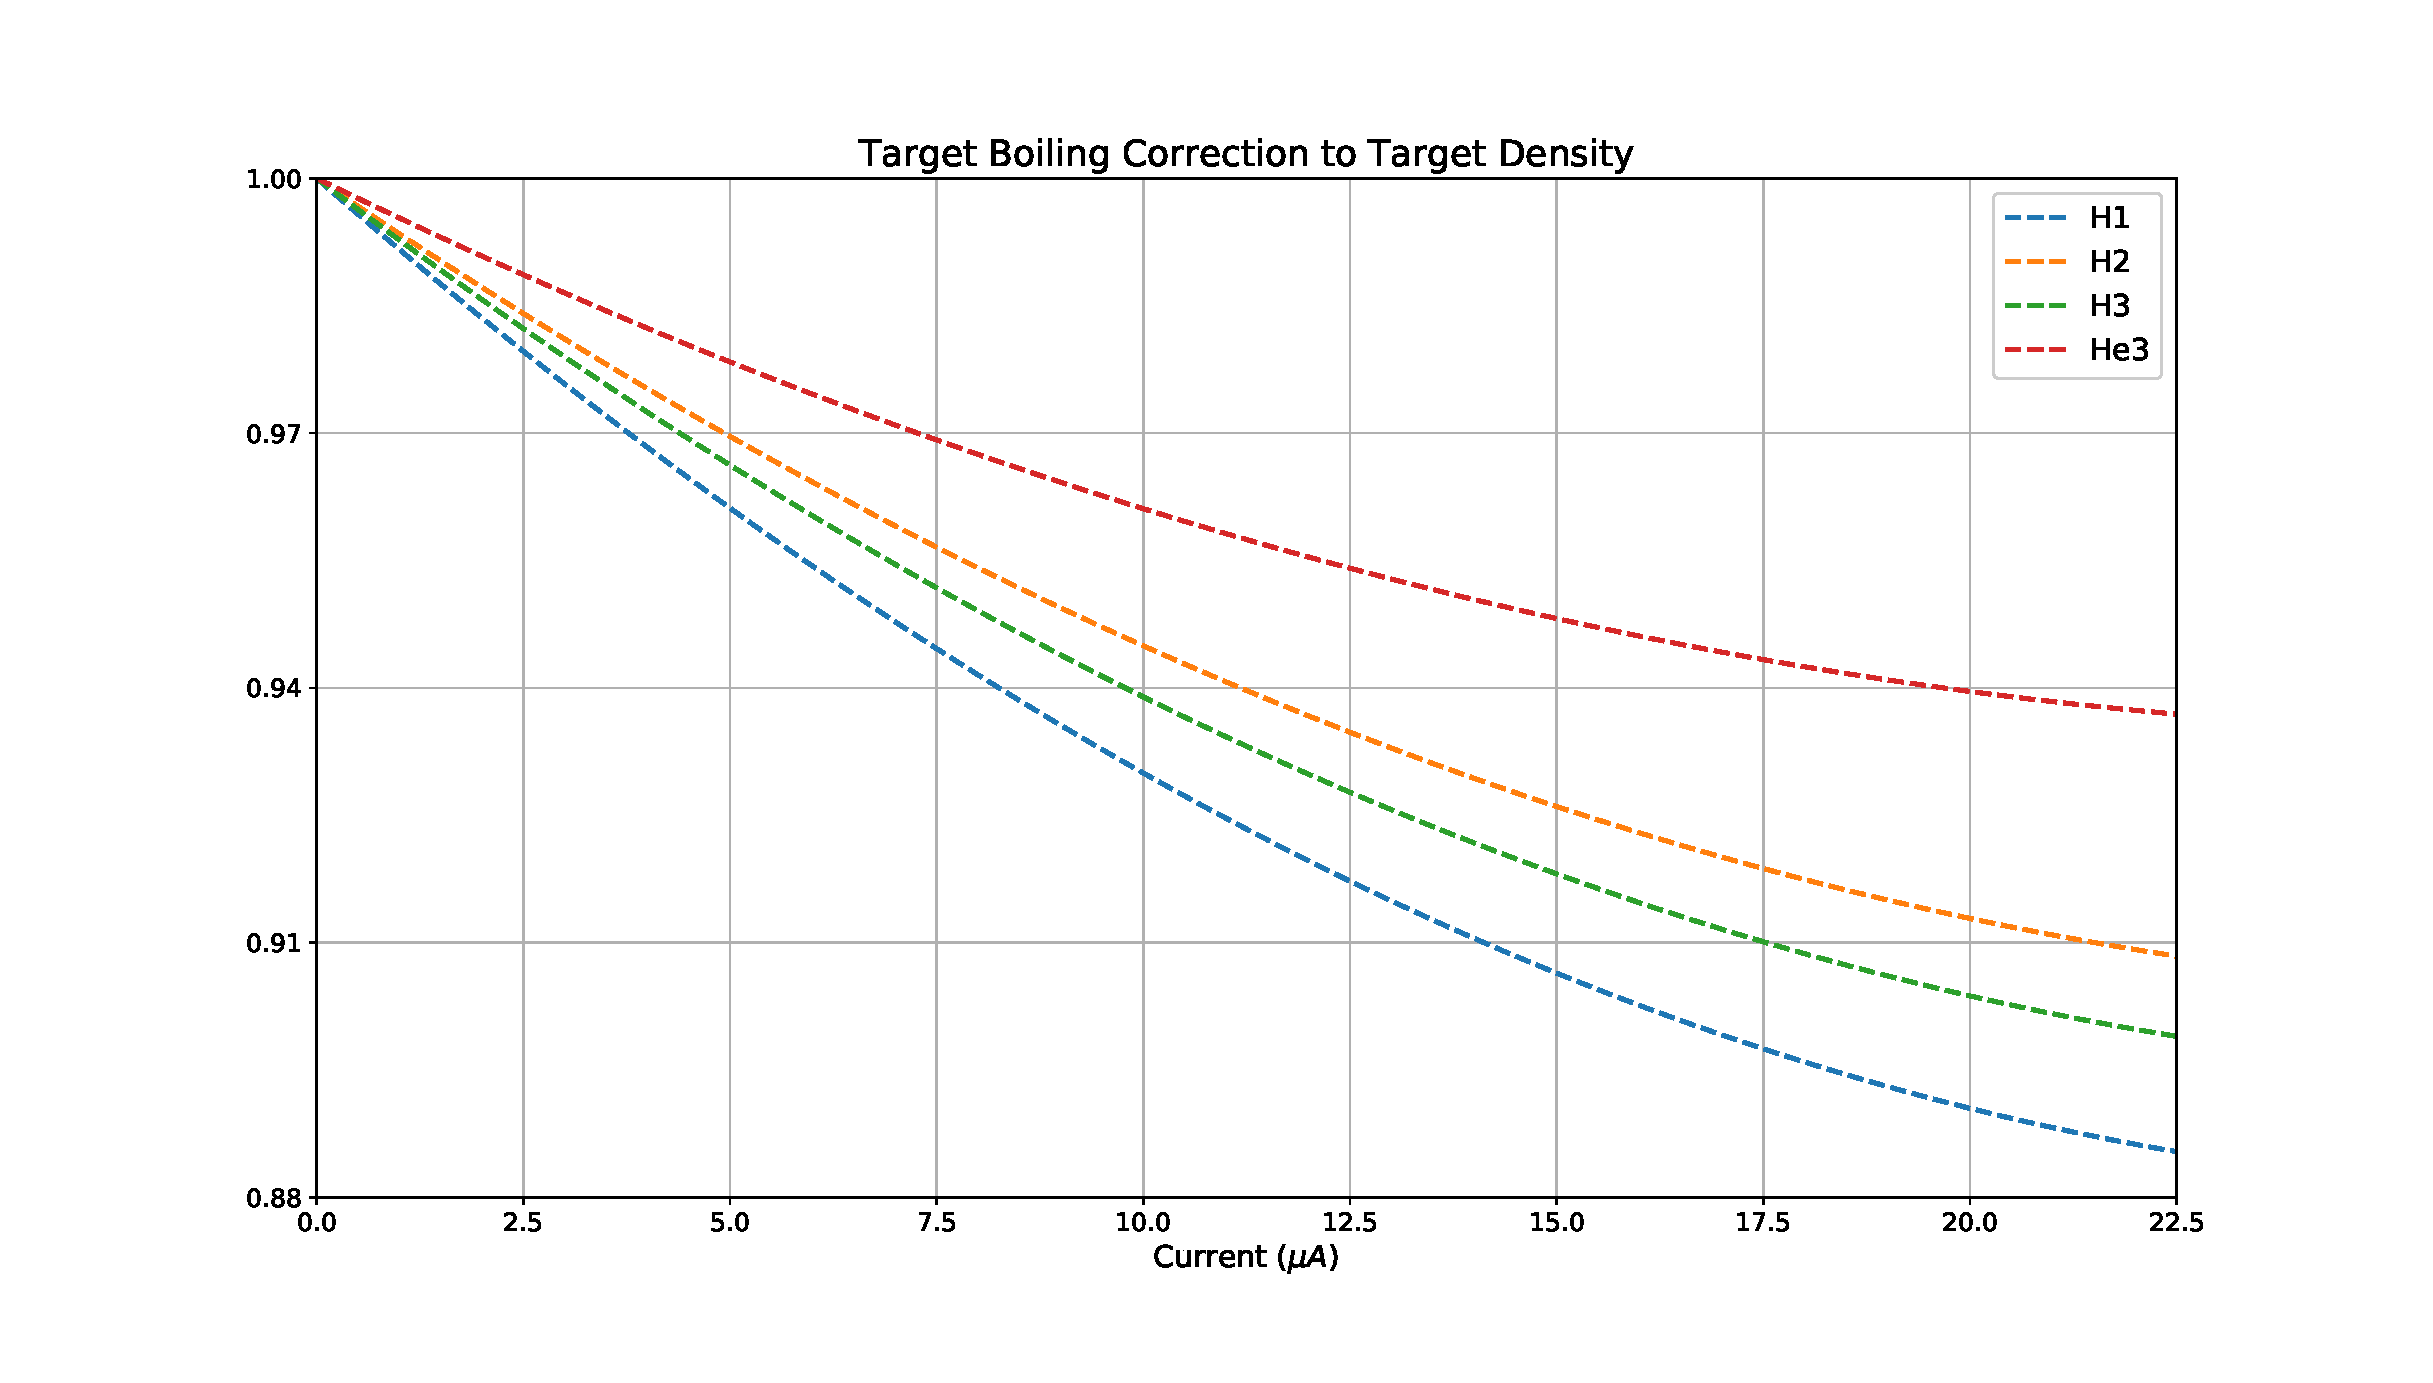
\includegraphics[width=\textwidth]{./chap3-analysis/fig/boil_cor.eps}
	\caption{Beam heating effects are manifested as a multiplicative correction to the target density}
	\label{fig:boilcor}
\end{figure}

\begin{figure}
	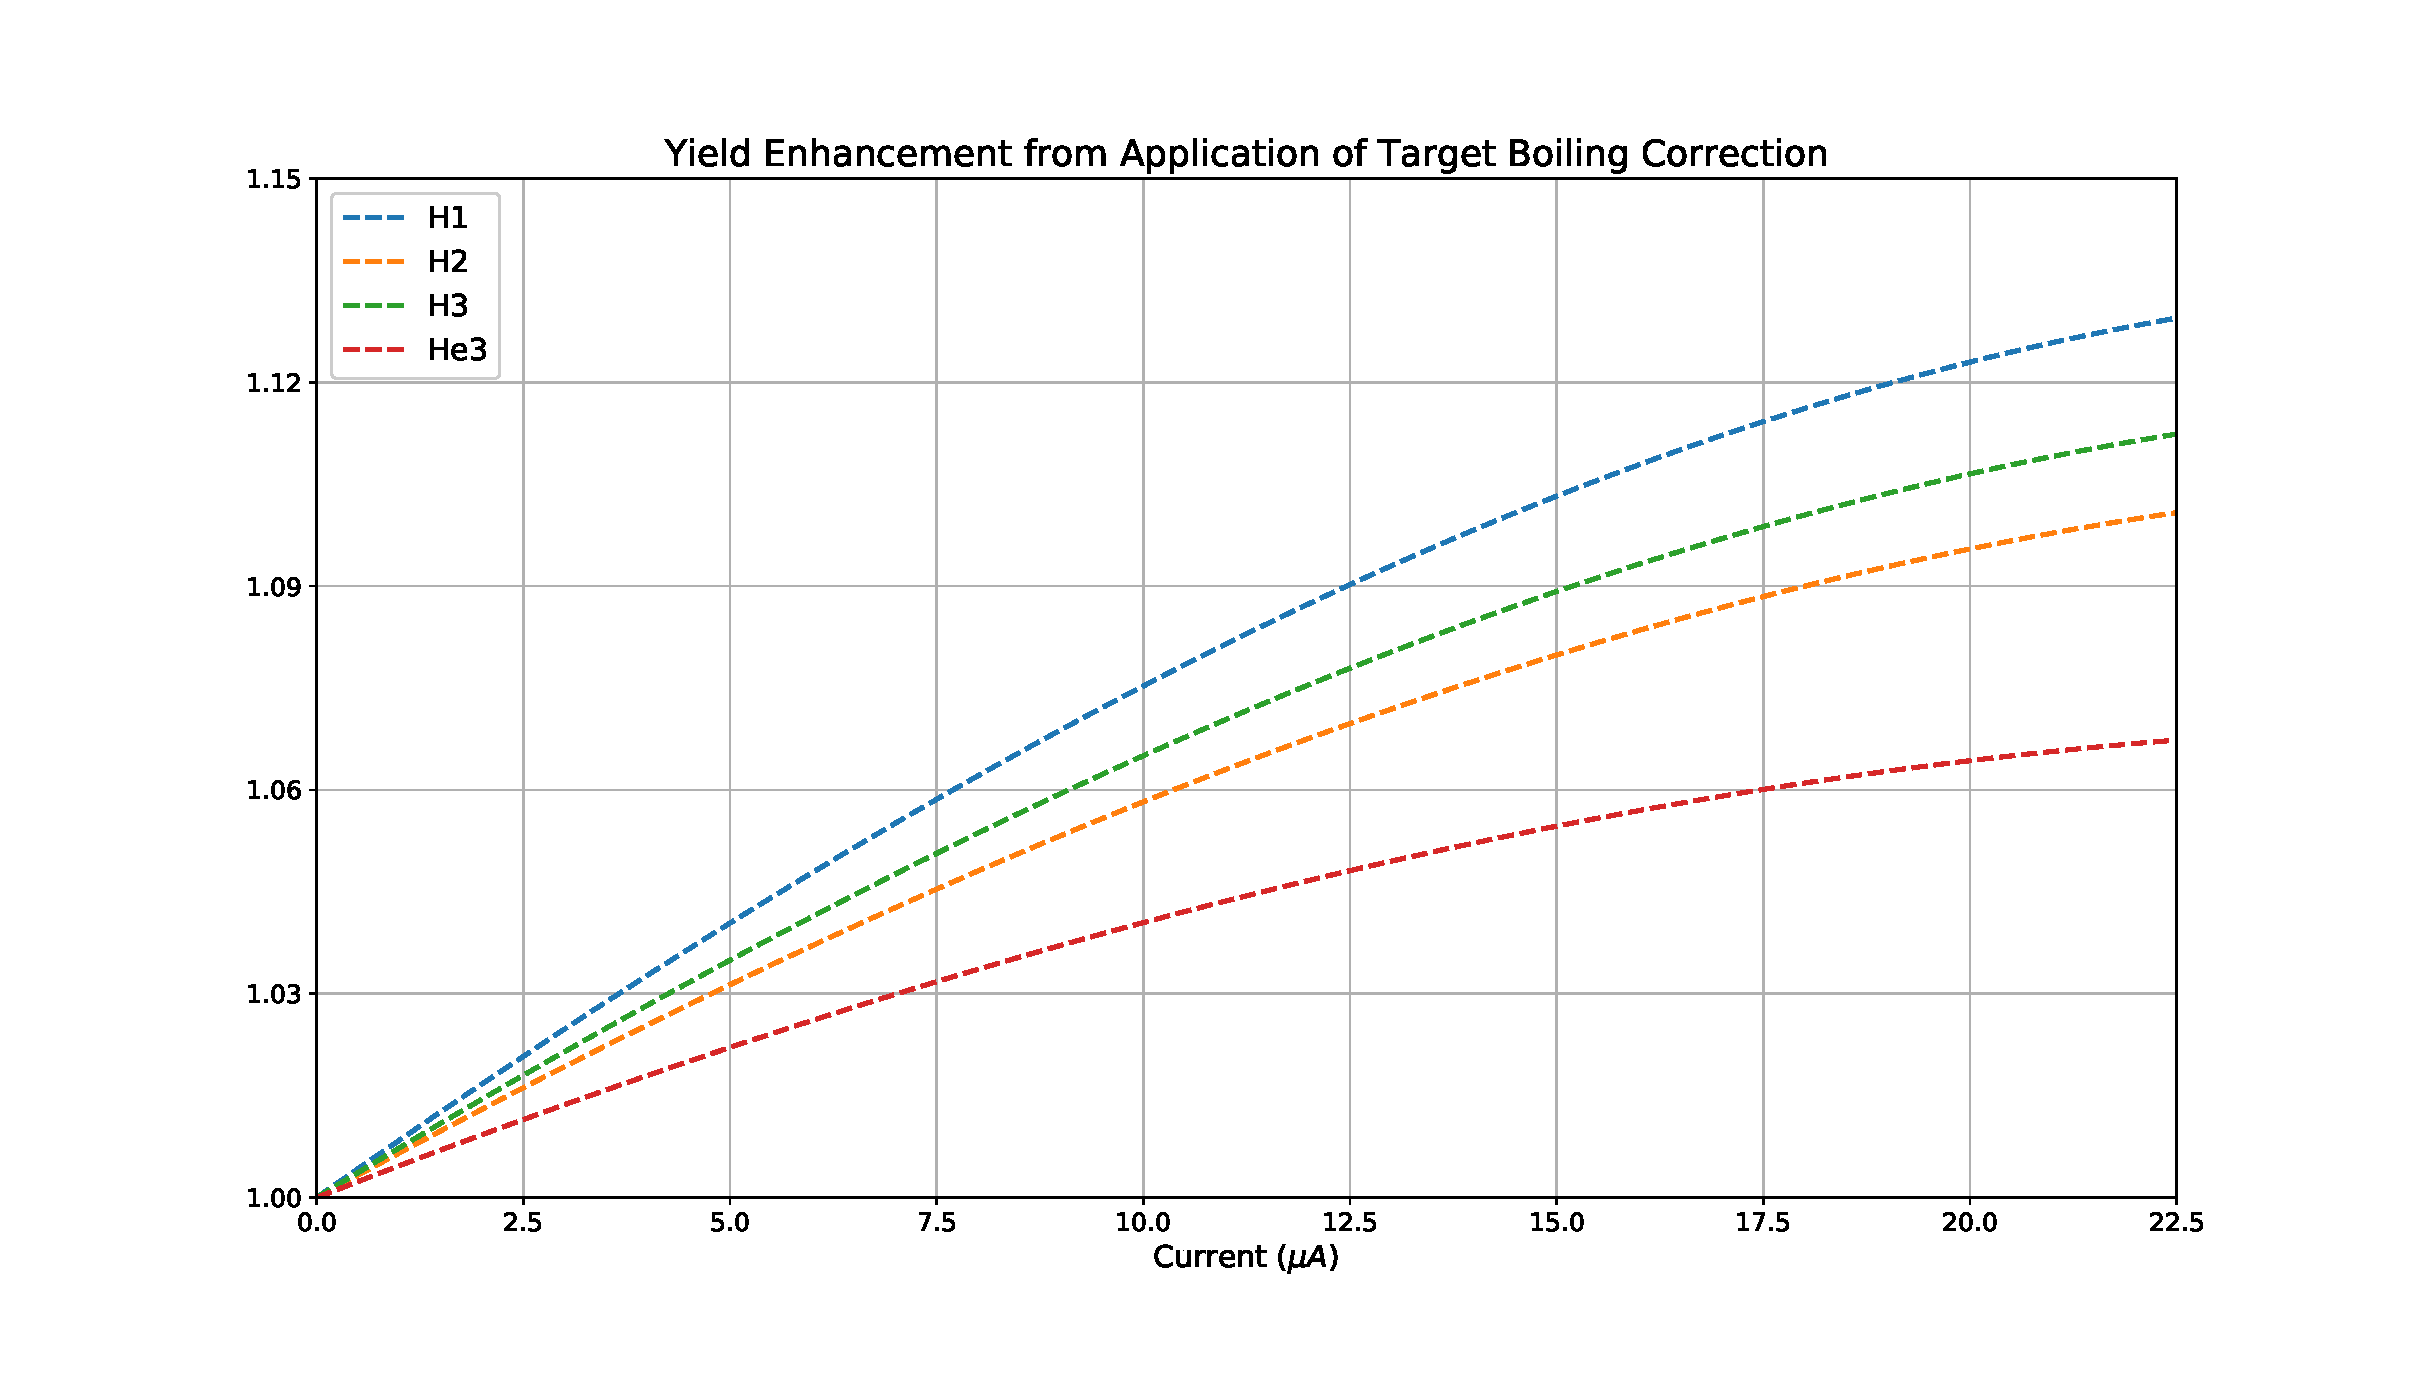
\includegraphics[width=\textwidth]{./chap3-analysis/fig/boil_yield_cor.eps}
	\caption{Target density corrections cause a multiplicative enhancement to the yield}
	\label{fig:boilyieldcor}
\end{figure}

\subsubsection{Target Endcap Contamination}

All of our gas targets are stored in an aluminum cell. The thickness of the aluminum greatly exceeds the thickness of the gas and will sometimes contribute background that makes it past our cuts. To determine this contribution, we use an empty cell. The empty cell, being an exact replica of the gas target cells with a vacuum inside, allows us to approximately isolate the contribution of the cell walls to the data.

To determine this contribution, the empty cell is normalized to the target in question. This is done by.........

The data for the target in question and the normalized empty target are then binned in Bjorken x. Dividing the empty cell data by the gas target data then gives an approximation of the fractional contribution of the cell walls to the electron data. This fractional contribution can be the subtracted from the charge normalized yields to correct for the data coming from the endcaps.

\subsubsection{Charge Symmetric Background Subtraction}

As an inclusive scattering experiment, we are particularly susceptible to background from charge symmetric processes from the target. To study this background we reversed the polarity of the Left HRS to take positron data at several low Bjorken x kinematics.

Measuring the positron yield allows us to determine the proportion of electron events measured that were a result of pair production. This data was subject to the same cuts that are used on the electron data. It was noted that a significant $\pi^+$ contamination occurred for the positron data. The main pion peak was fit and then subtracted from the positron data.

These data were then binned by Bjorken x and fit with an exponential. 

Somethin somethin somethin... Provide x of bin and multiply by $1-\mathrm{curve}$.

\begin{figure}
	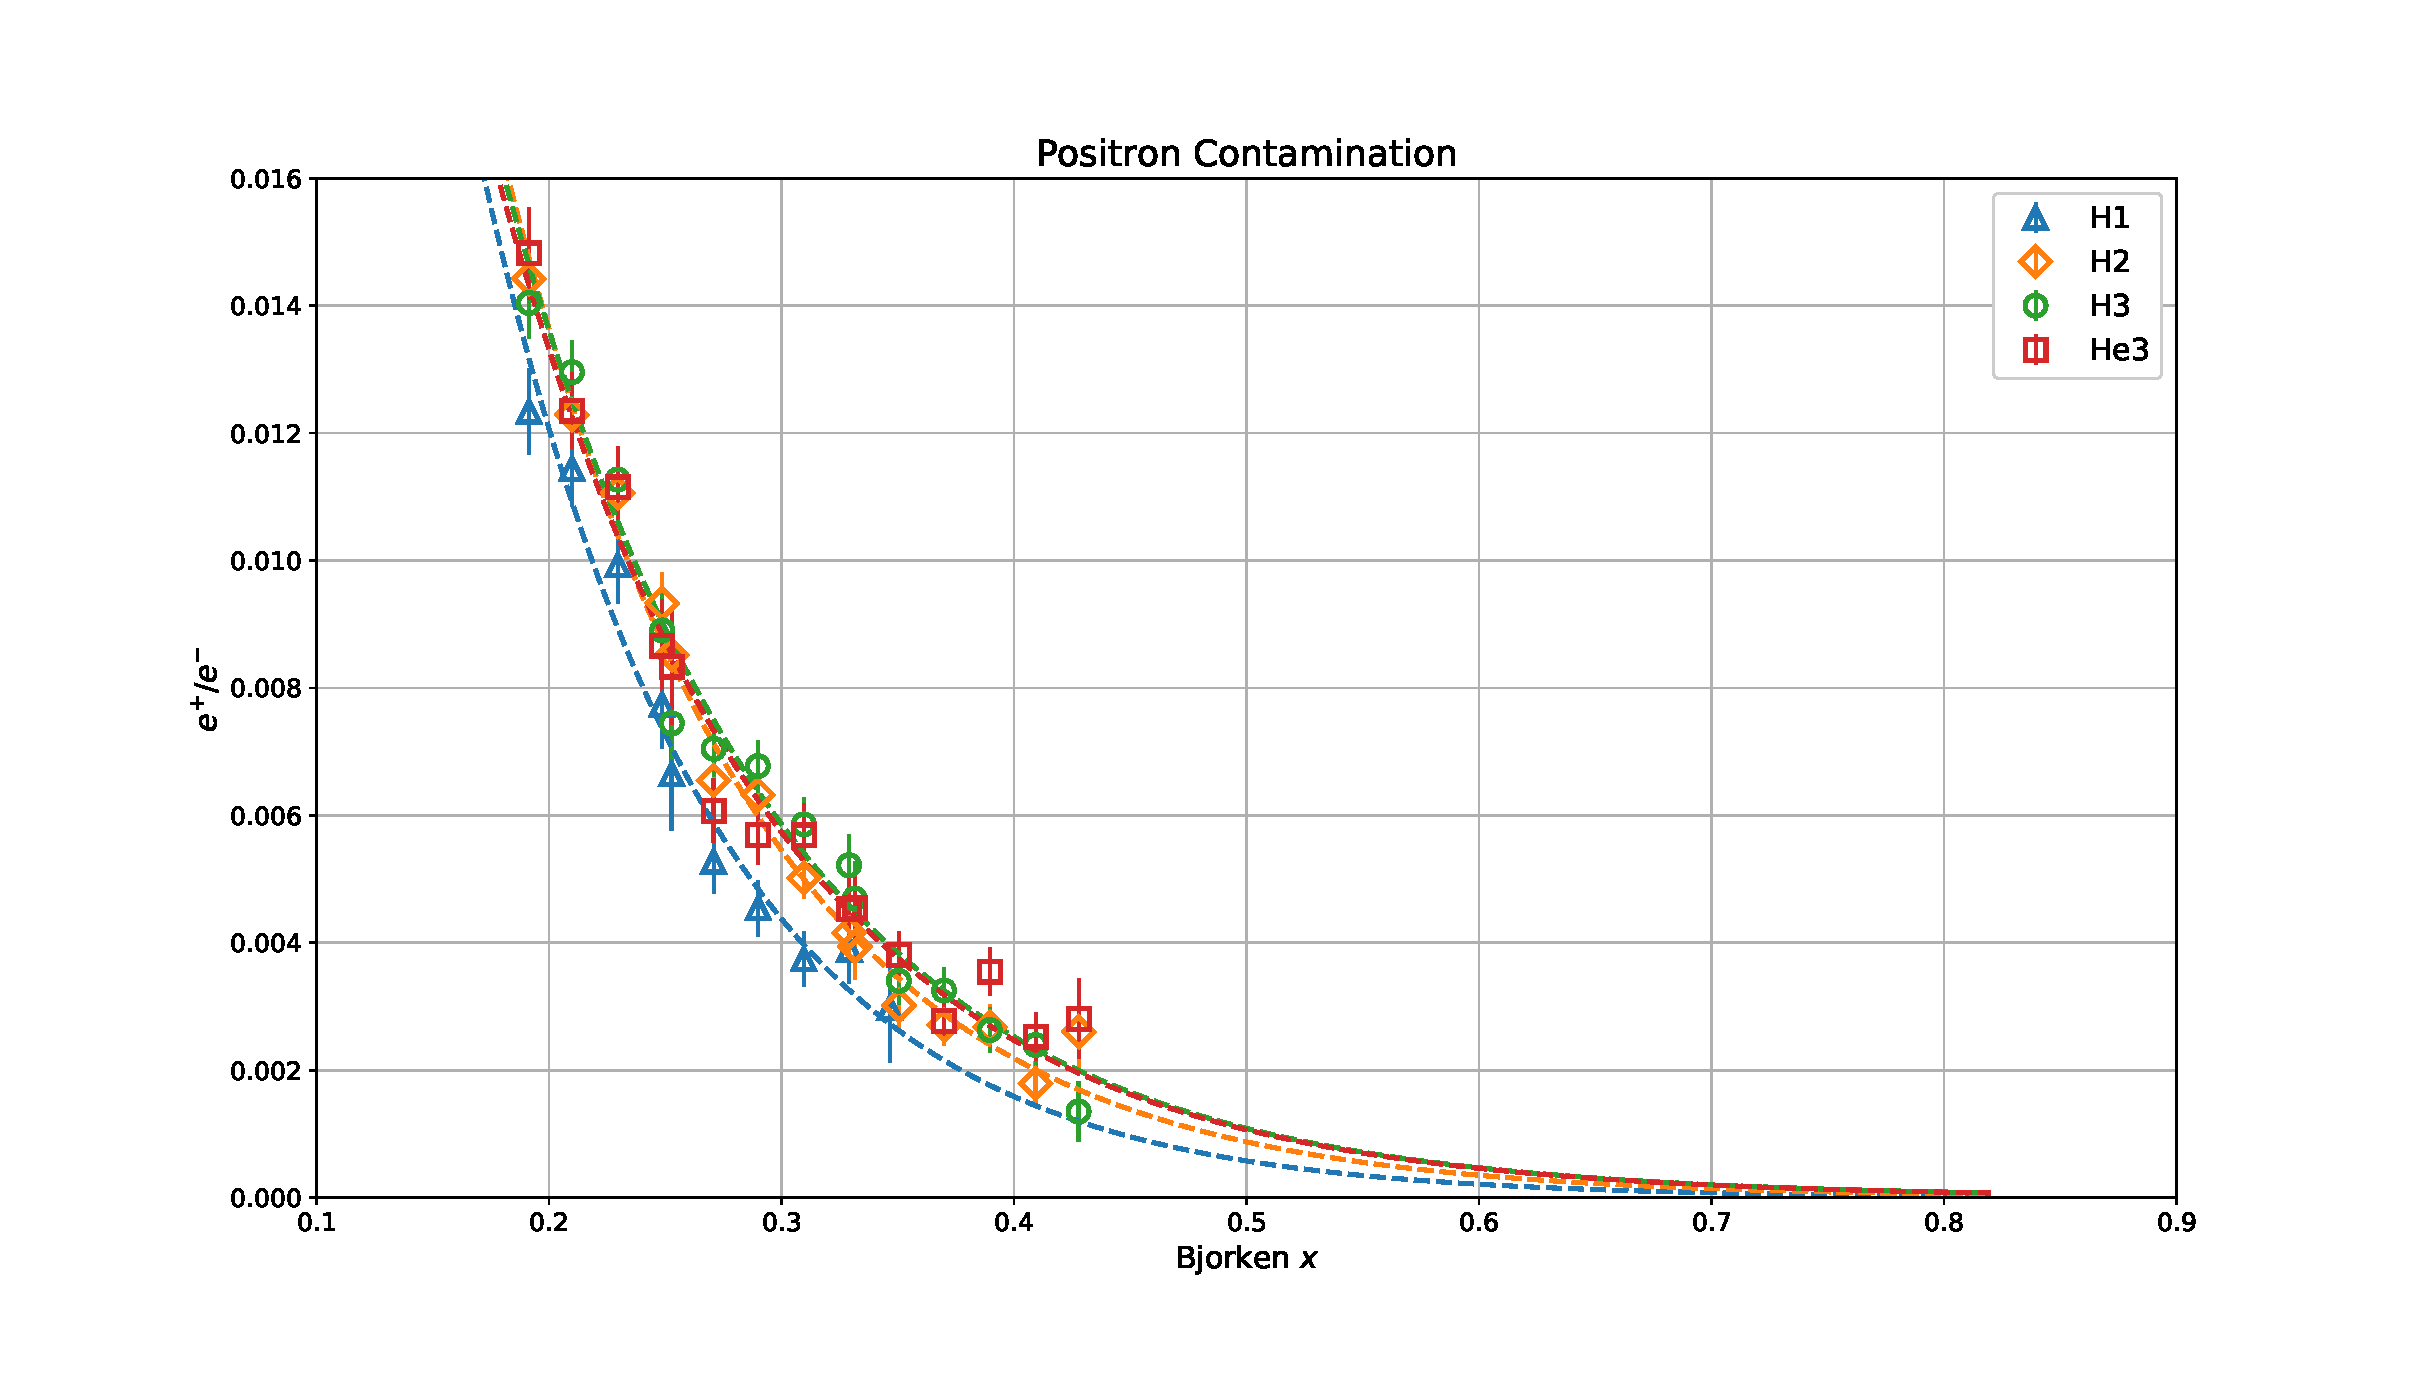
\includegraphics[width=\textwidth]{./chap3-analysis/fig/positrons.eps}
	\caption{Charge symmetric background correction}
	\label{fig:positrons}
\end{figure}

\subsubsection{Computer Deadtime Correction}

Our DAQ unable to be continuously taking data. While we can probabilistically determine the mean time spacing between events, in the real world events can deviate greatly from these means \textbf{because statistics}. Sometimes events will occur that are too close in time for our DAQ to record all of them. When deadtime becomes significant, we must correct for it.

An approximation of the computer deadtime was measured with our scalers. The trigger signals generated by the NIM electronics were copied and sent to both the Trigger Supervisor and a scaler unit. The Trigger Supervisor is subject to the computer deadtime event loss discussed here. The scaler unit simply increments a register when a trigger signal is received. The deadtime is defined on a run-by-run basis as:

\begin{equation}
DT = 1 - \frac{\Sigma \mathrm{Triggers_{TS}}}{\Sigma \mathrm{Triggers_{Scaler}}}
\end{equation}

A deadtime correction is applied on a run-by-run basis. The correction is defined as:

\begin{equation}
DT_{\mathrm{correction}} = \frac{1}{1-DT}
\end{equation}

\begin{figure}
	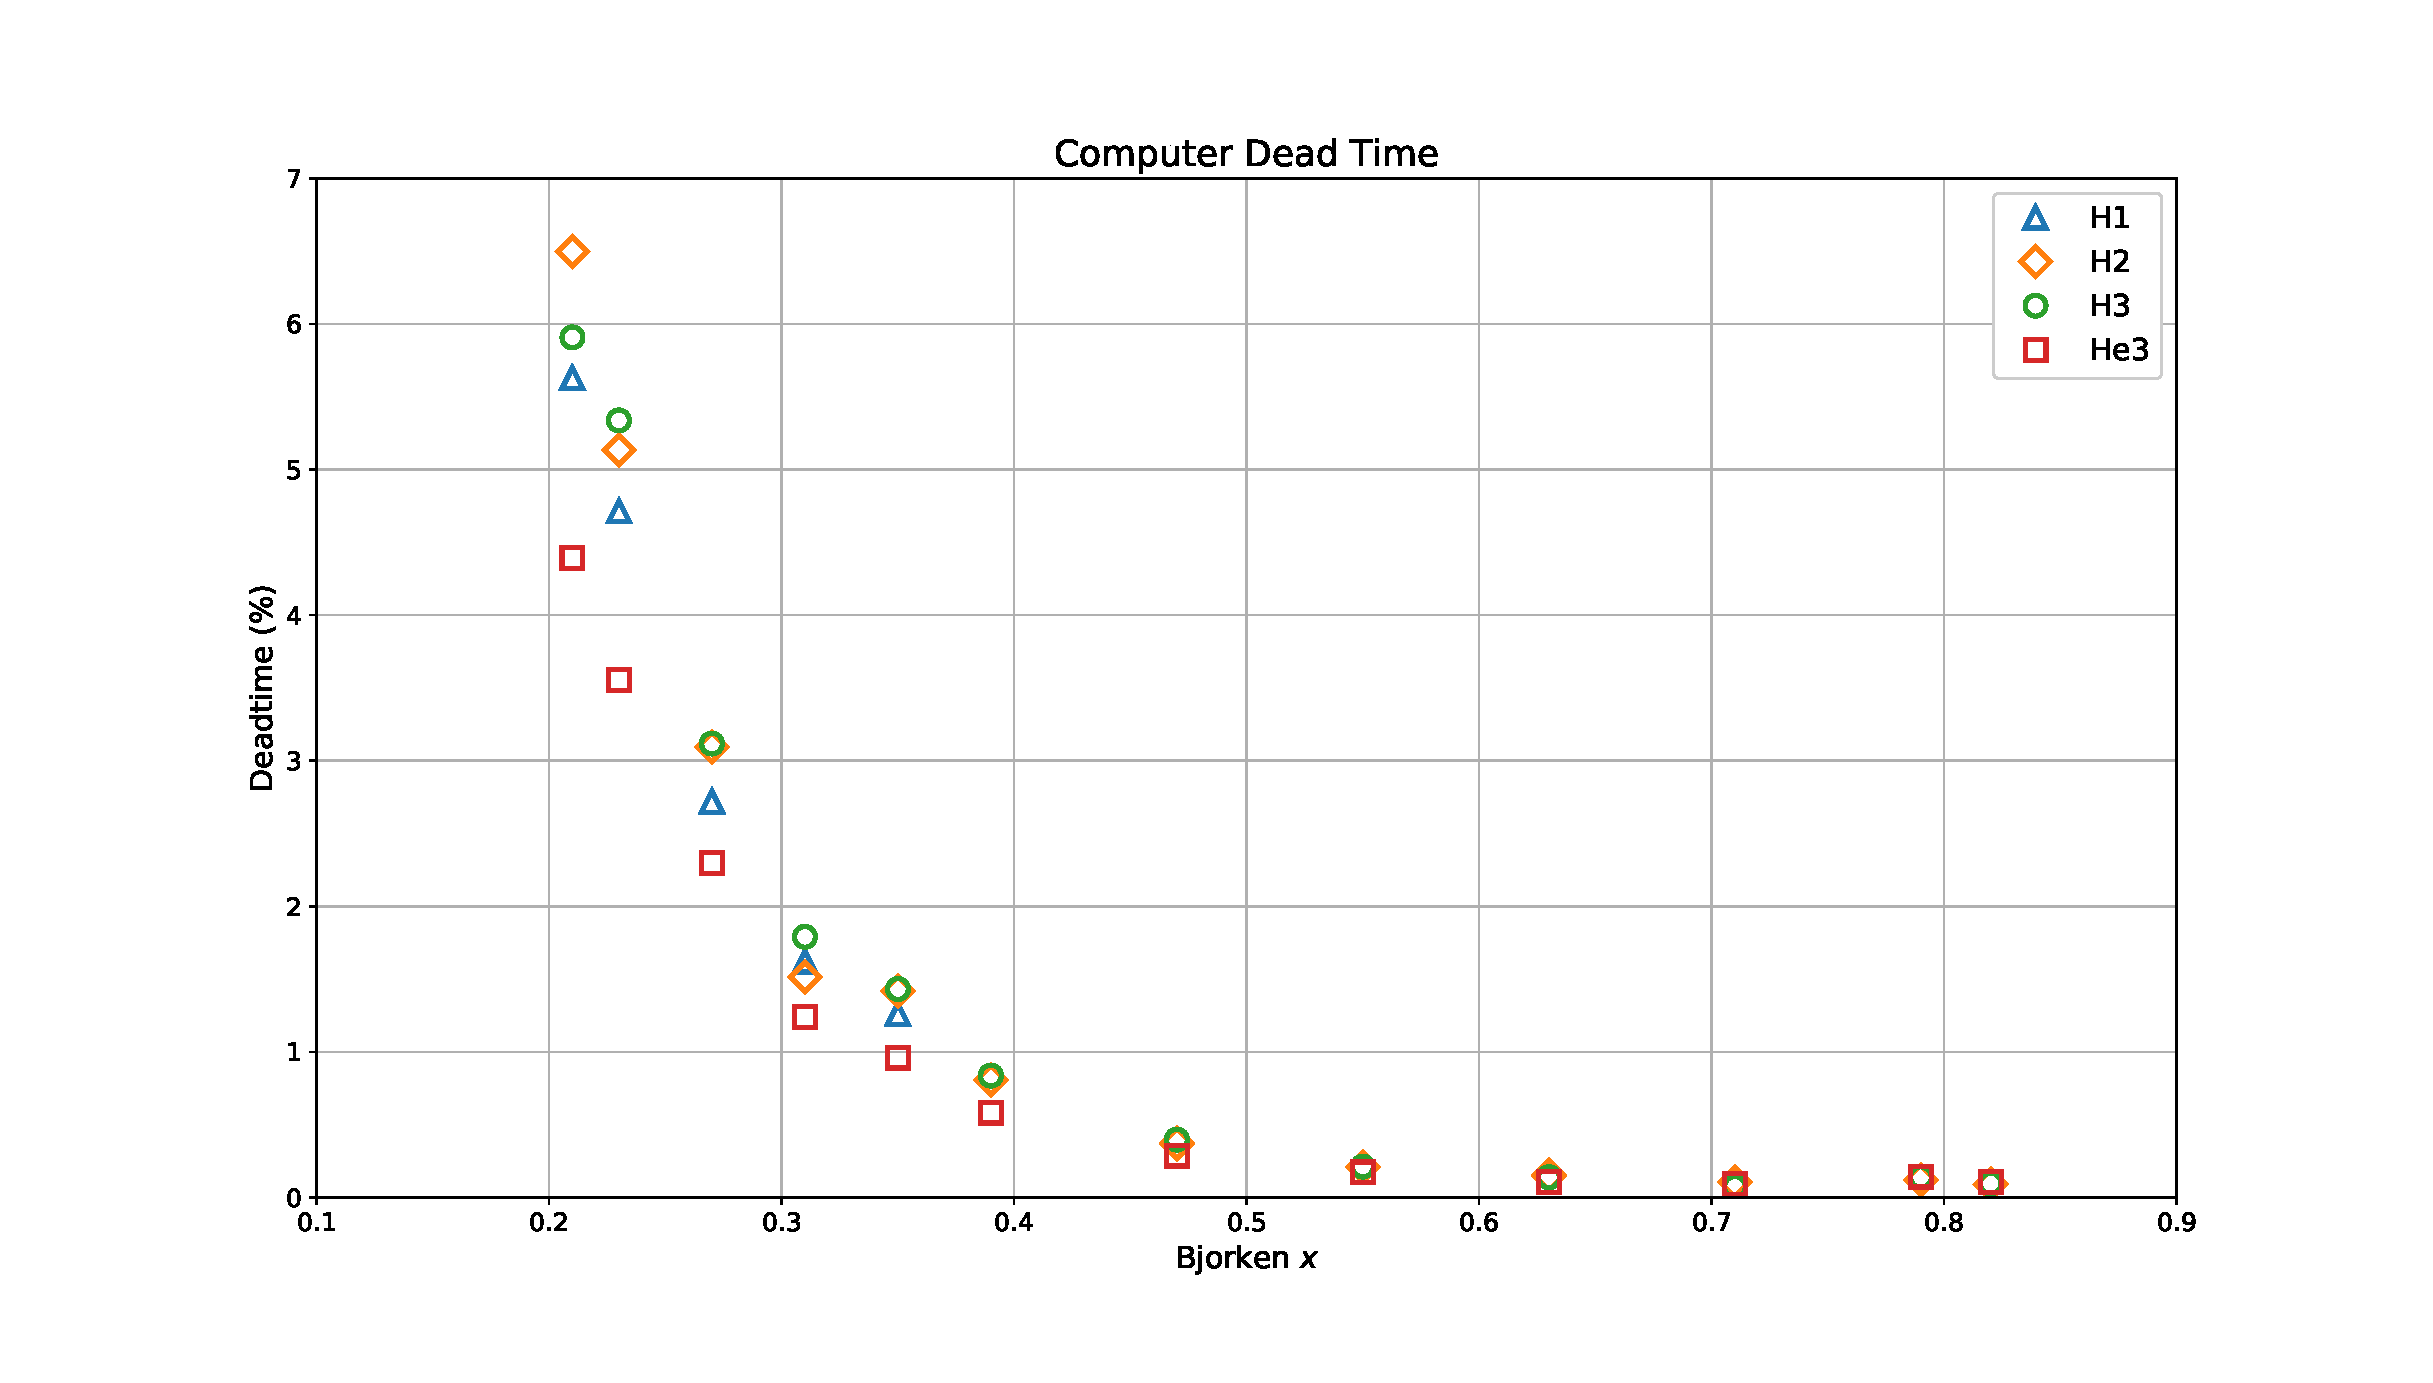
\includegraphics[width=\textwidth]{./chap3-analysis/fig/deadtime.eps}
	\caption{Deadtime per kinematic}
	\label{fig:deadtime}
\end{figure}

\subsubsection{Radiative Corrections}

\subsubsection{Isoscalar Corrections}

\subsubsection{Bin Centering Corrections}

\subsubsection{Coulomb Corrections}